\documentclass[12pt,letterpaper]{lsuetd}
\usepackage{setspace,graphics,dsfont,verbatim,paralist,indentfirst,amsmath}
\usepackage{tabularx}
\usepackage{empheq}
\usepackage{color}
\usepackage[table]{xcolor}
\usepackage{colortbl}
\usepackage{rotating}
\usepackage{fancyref}
\usepackage{hyperref}
\usepackage[final]{pdfpages}
\setlength{\topmargin}{-0.5in}
\setlength{\textheight}{9.0in}
\addtolength{\evensidemargin}{-0.50in}
\addtolength{\oddsidemargin}{-0.50in}
\addtolength{\textwidth}{1.00in}
\setlength{\parindent}{1.75em}
\setlength{\parskip}{0ex}
\setcounter{tocdepth}{2}

%\renewcommand{\end{equation}}{\end{equation}\vspace{12pt}}

\newenvironment{equations}{\vspace{6pt}\begin{equation}}{\end{equation}\vspace{3pt}}



\definecolor{red}{RGB}{128,0,0}
\hypersetup{
  colorlinks,
  citecolor=red,
  filecolor=red,
  linkcolor=red,
  urlcolor=red
}

\definecolor{Gray}{gray}{.9}
\newcommand\y{\cellcolor{gray!10}}
\newcommand{\logit}{\mathrm{logit}}


\usepackage{titlesec}

\usepackage{etoolbox}
\makeatletter
\patchcmd{\ttlh@hang}{\parindent\z@}{\parindent\z@\leavevmode}{}{}
\patchcmd{\ttlh@hang}{\noindent}{}{}{}
\makeatother

\titlespacing*{\section}
{0pt}{36pt}{24pt}
\titlespacing*{\subsection}
{0pt}{30pt}{24pt}
\titlespacing*{\subsubsection}
{0pt}{20pt}{16pt}

%\titleformat*{\subsubsection}{\large\bfseries\thesection.\thesubsection}
\titleformat*{\subsubsection}{\large\bfseries}

\makeatletter

\setlength{\abovedisplayskip}{3em}
\setlength{\belowdisplayskip}{3em}
\setlength{\abovedisplayshortskip}{3em}
\setlength{\belowdisplayshortskip}{3em}

\begin{document}
\renewcommand\@pnumwidth{1.55em}
\renewcommand\@tocrmarg{9.55em}
\renewcommand*\l@chapter{\@dottedtocline{0}{1.5em}{2.3em}}
\renewcommand*\l@figure{\@dottedtocline{1}{0em}{3.1em}}
\let\l@table\l@figure

\pagenumbering{roman}
\thispagestyle{empty}
\begin{center}
%The title page is first created.
A GRAPH-BASED TAXONOMIC INTELLIGENT TUTORING SYSTEM UTILIZING 
BLOOM'S TAXONOMY AND ITEM-RESPONSE THEORETIC ASSESSMENT

\vfill
\doublespacing
A Thesis/Dissertation \\
\singlespacing
Submitted to the Graduate Faculty of the \\
Louisiana State University and \\
Agricultural and Mechanical College \\
in partial fulfillment of the \\
requirements for the degree of \\
Ph.D. \\
\doublespacing
in \\
                                       
Computer Science \\
\singlespacing
\vfill

by \\
Dennis Castleberry \\
B.S., LSU, 2009 \\
May 2017
\end{center}
\pagebreak
%The Copyright Page and Dedication sections can be added here, if desired.

%\chapter*{Copyright Page}
%\doublespacing
%\vspace{0.55ex}
%Insert the appropriate text for the copyright page here.
%\addcontentsline{toc}{chapter}{\hspace{-1.5em} {COPYRIGHT PAGE} \vspace{12pt}}
%\pagebreak

%\chapter*{Dedication}
%\doublespacing
%\vspace{0.55ex}
%Insert the appropriate text for the dedication or epigraph page here.  This part of the ETD must not exceed one page.
%\addcontentsline{toc}{chapter}{\hspace{-1.5em} {DEDICATION} \vspace{12pt}}
%\pagebreak

\chapter*{Acknowledgments}
\doublespacing
\vspace{0.55ex}

I would like to thank my research group, my committee, and the Department of
Computer Science for supporting my teaching and research efforts throughout
my career.

%The code below adds the Acknowledgments section to the Table of Contents.
\addcontentsline{toc}{chapter}{\hspace{-1.5em} {ACKNOWLEDGMENTS} \vspace{12pt}}
\pagebreak
%The Preface section can now be added, if desired.

%\chapter*{Preface}
%\doublespacing
%\vspace{0.55ex}
%Insert the appropriate text for the preface here.
%\addcontentsline{toc}{chapter}{\hspace{-1.5em} {PREFACE} \vspace{12pt}}
%\pagebreak

\singlespacing
\tableofcontents
\pagebreak

%The code below generates the List of Tables and adds it to the Table of Contents.
\renewcommand\@pnumwidth{1.55em}
\renewcommand\@tocrmarg{8.55em}
\addcontentsline{toc}{chapter}{\hspace{-1.5em} LIST OF TABLES \vspace{12pt}}
\listoftables
\pagebreak
%The code below generates the List of Figures and adds it to the Table of Contents.
\addcontentsline{toc}{chapter}{\hspace{-1.5em} LIST OF FIGURES \vspace{12pt}}
\listoffigures
\pagebreak
%The List of Nomenclature may be included here, if desired.

%\chapter*{List of Nomenclature}
%\doublespacing
%\vspace{0.55ex}
%Provide the definitions of the symbols used in your thesis or dissertation here.
%\addcontentsline{toc}{chapter}{\hspace{-1.5em} LIST OF NOMENCLATURE \vspace{12pt}}
%\pagebreak

%The code below adds the Abstract and places it within the Table of Contents.
\renewenvironment{abstract}{{\hspace{-2.2em} \huge \textbf{\abstractname}} \par}{\pagebreak}
\addcontentsline{toc}{chapter}{\hspace{-1.5em} ABSTRACT}
\begin{abstract}
\vspace{0.55ex}
\doublespacing

This dissertation details an intelligent tutoring system which aims to raise
student trait abilities across concepts and levels of Bloom's taxonomy within
an educational program.  

The system utilizes Item Response Theory, a probabilistic theory of assessment
which accounts for item discrimination, difficulty, and probability of guessing
in its assessment of student trait ability.

The intelligent tutoring system features a graph-based model of dependency
relationships among questions, models of memory and forgetting, and
fine-grained characterization-based models of student ability.  In conjunction,
these lend to efforts to schedule problems for the particular student which
have the highest payoff.

\end{abstract}

\pagenumbering{arabic}
\addtocontents{toc}{\vspace{12pt} \hspace{-1.8em} CHAPTER \vspace{-1em}}
\singlespacing
\setlength{\textfloatsep}{12pt plus 2pt minus 2pt}
\setlength{\intextsep}{6pt plus 2pt minus 2pt}
\chapter{Background Information}
\doublespacing

\section{Introduction}

\subsection{Problem Definition}

A \emph{content item} is some unit of information, such as a statement, graph,
table, example, and so forth.  An educationl television program, interactive
tutorial or university lecture (generally, these may all be called programs)
can be broken down into these units of information.  Call an item $\chi$; then
the $i^{th}$ item to be seen is $\chi_i$, and the time at which it is seen
$t_i$.  Then $(\chi_i, t_i)$ represents the $i^{th}$ item and its scheduled
time.  

For that matter, any program can be thought of as a sequence of these tuples,
thereby forming a schedule of items: 

\begin{equations}
\label{eq:schedule}
   X = \langle (\chi_1, t_1), (\chi_2, t_2), \ldots (\chi_n, t_n) \rangle.
\end{equations}
\vspace{2pt}

Furthermore $\chi$ could be a question, which could be thought of as an item
which accepts a response back that has a correct answer.  Items and questions
share many similar properties which help to distinguish them, such as the
ones in Fig~\ref{fig:properties}.

The main question this body of work seeks to answer is this: \emph{based on
input from the student on any subset of questions in an item schedule, how
should the remaining questions be scheduled}?

\subsection{Novel Contributions}

The answer to this question required a series of novel contributions to the
fields of intelligent tutoring systems (ITS) and computer-aided assessment
(CAT).  Specifically:

\begin{itemize}

 \item The creation of a data structure in the form of a graph, whose nodes
 contain information relevant to the assessment process, and whose edges
 capture dependency relationships among questions;

 \item A modification to an existing assessment theory known as Item Response
 Theory, which however providing a mature means of assessing student ability,
 benefited from an account of dependency relationships;
 
 \item A scheduler, or algorithm whose purpose was to determine what the
 questions should be given the item parameters and the students' response
 sets;

 \item An addendum to an existing theory of memory, forgetting, and practice,
 which could then be integrated into the scheduler to provide a fuller-featured
 system.

\end{itemize}

In addition to this, the body of work rests upon other incidental novel
contributions, such as the separation of Bloom level and difficulty
\cite{castleberry}.

\section{Bloom's Taxonomy}

Bloom's cognitive taxonomy organizes questions into levels depending on the
cognitive functions required of the answerer.  The levels are: knowledge,
comprehension, application, analysis, evaluation, and synthesis.  A brief
overview is given in Table~\ref{tab:bloom}, with definitions and examples of
questions covering the concept of for-loops:

\begin{table}[!p]
\label{tab:bloom}
\caption{The levels of Bloom's taxonomy defined}
\vspace{12pt}
\begin{tabularx}{\textwidth}{||l|X|X||}
\hline \hline
\rowcolor{Gray}
Level &  Explanation & Example Question \\\hline
Knowledge & Recalling factual information.   
& {What is a for-loop?}
\\ \hline
Comprehension & Assigning meaning to information.   
& {What does the example for-loop output? (Give example.)}
\\ \hline
Application & Applying a rule to a specific instance.   
& {How can the update statement of the loop be changed to print 
only even numbers?}
\\ \hline
Analysis 
& Breaking information into parts and exploring relationships.   
& {What would happen if the update statement decremented instead of incremented the counter?}
\\ \hline
Evaluation 
& Judging the use of knowledge or the validity of an
argument.   
& {Which is better for reading user input: a for-loop or a
while-loop? Why?} 
\\ \hline
Synthesis 
& Utilizing knowledge to create a new solution to
satisfy a goal.   
& {Write a for-loop to print only even numbers up to ten.}
\\ \hline \hline 
\end{tabularx}
\vspace{36pt}
\end{table}

\begin{table}[!p]
\label{tab:grades}
\caption{Grades mapped to trait ability levels}
\vspace{12pt}
\begin{tabularx}{\textwidth}{||l|c|X||}
\hline\hline
\rowcolor{Gray}
Letter  & $\theta$  & Explanation \\\hline
F  & -3.0   & unsatisfactory \\\hline
D- & -2.5   &                \\
D  & -2.0   & minimal        \\
D+ & -1.5   &                \\\hline
C- & -1.0   &                \\
C  & -0.5   & acceptable     \\
C+ & 0.0    &                \\\hline
B- & 0.5    &                \\
B  & 1.0    & good           \\
B+ & 1.5    &                \\\hline
A- & 2.0    &                \\
A  & 2.5    & distinguished  \\
A+ & 3.0    &                \\\hline\hline
\end{tabularx}
\vspace{36pt}
\end{table}


Each category depends on the cognitive functions used in the previous category.
That is, comprehension requires knowledge, application requires comprehension,
and so forth.  Furthermore the mastery of one of the levels is with respect to
a given concept.  A student may be able to synthesize solutions to problems
dealing with expressions, but may not possess knowledge of equations, and thus
could not solve problems involving equations.

The utility of Bloom's taxonomy lies in its ability to pinpoint the underlying
cause of the student's problem-solving impasses \cite{shuhidan2011}.  
There is even evidence to suggest that Bloom levels correspond to different
electroencephalographic (EEG) signatures \cite{chatterjee2015}, implicating
distinct brain functions in their use. 

Suppose a test of mastery of loops is given with the comprehension question
``What does such-and-such loop output?'' is given, and the student reaches an
impasse.  If the question ``What are the three expressions of the loop and what
do they do?'' is asked and the student does not know, the impasse can be
attributed to a lack of knowledge about loops.  If the student does know about
the loop expressions but still cannot answer, one might instead attribute it to
a comprehension difficulty \emph{as such}; which might be remedied by giving
some examples to build intuition, then continuing to test at the comprehension
level.

Educators may have an intuitive notion of how to do this, but Bloom's taxonomy
gives the ability to examine the impact of questions scientifically.  By
identifying the tested concept and the Bloom level of exercises, one can then
form hypotheses about student responses to questions.  

\subsection{The Interpretation in Computer Science}

Bloom's taxonomy has been proven to be useful at the undergraduate level, and
particularly in the field of software engineering \cite{britto2015,
mahmood2014}.  It has seen success in program comprehension
\cite{buckley2003}, where the asking of comprehension questions fosters code
reading \cite{losada2008}. In addition, it has been useful for pinpointing the
difficulties of novice programmers in a guided learning approach
\cite{shuhidan2011}.  It been used to identify a marked preference for
higher-level problems for those able to solve them \cite{bruyn2011}
\cite{goel2004}.  At least two experiments have shown the effect of item
ordering on performance \cite{newman1988effect,castleberry2016effect}, and the
taxonomy has even been applied to create ratings of courses based on the
average Bloom levels of tasks and questions in the course
\cite{oliver2004course}.

In spite of all this, there is an ongoing debate regarding the applicability of
Bloom's taxonomy to computer science \cite{johnson2006bloom,
fuller2007developing, thompson2008bloom}.  The crux of this debate centers
around the interpretation of Bloom levels: not only how questions map to Bloom
levels, but also regarding the progression of Bloom levels over the span of a
course or curriculum.  

A tacit assumption in much of the research is that Bloom levels equate to
difficulty levels.  While there is certainly a relationship between Bloom level
and difficulty in the ``ordinary course'' of devising problems, a distinction
can be made between the two.
% TODO: (SRB) cite the papers you cite in the difficulty paper regarding this
% assumption.

\subsection{Assumptions of this Work}

% TODO: (SRB) cite the prior research. I know it's not published yet.
Prior research by the author supports the view that Bloom level and difficulty
are separable parameters of a content item.  This work will proceed on the
assumption to that effect. 

In addition, some of the components of this body of work, particularly those
pertaining to memory and recall, are supported by many decades of empirical
research \cite{ebbinghaus}.  While the study of intelligent tutoring systems
has seen attempts to validate addendums to these theories which accommodate
re-activation of forgotten knowledge, none have undergone extensive empirical
testing as is typical for psychological models.  The components of this body of
work regarding re-activation introduce hypotheses.

\section{Item Response Theory}

Here is introduced a mature assessment theory known as Item Response Theory, an
alternative to Classical Test Theory (CCT).  Whereas Classical Test Theory
assigns a student a grade based on the student's position in a distribution of
composite test scores, Item Response Theory accounts for item difficulty, item
discrimination, the probability of guessing the question correctly.

One of the main appeals of IRT is its incorporation of item difficulty.  As
will be shown later, this is pertinent to the interpretation of Bloom levels.  

According to Item Response Theory (IRT), in what is known as the 3PL or 3
parameter logistic model, the probability $p_i$ that a student answers
correctly the $i^{th}$ question on a test, is given by:

\begin{equations}
 \label{eq:irt}
  p_i(\theta_s) = \gamma_i + \frac{1-\gamma_i}{1+e^{\alpha_i(\theta-\beta_i)}}
\end{equations}

where:

\begin{itemize} 

 \item $\alpha$ is the item discrimination, or how well the item can
 distinguish students of varying trait ability;

 \item $\beta$ is the question difficulty, 

 \item $\gamma$ is the probability of guessing the answer correctly,

 \item and $\theta$ is the \emph{trait ability} of the student, or the
 student's particular ability to answer that question correctly.

\end{itemize} 

A graph of the IRT curve for the parameters $\alpha=1, \beta=0, \gamma=0$ is
shown \ref{fig:irt}.

\begin{figure}[p!]
 \label{fig:irt}
 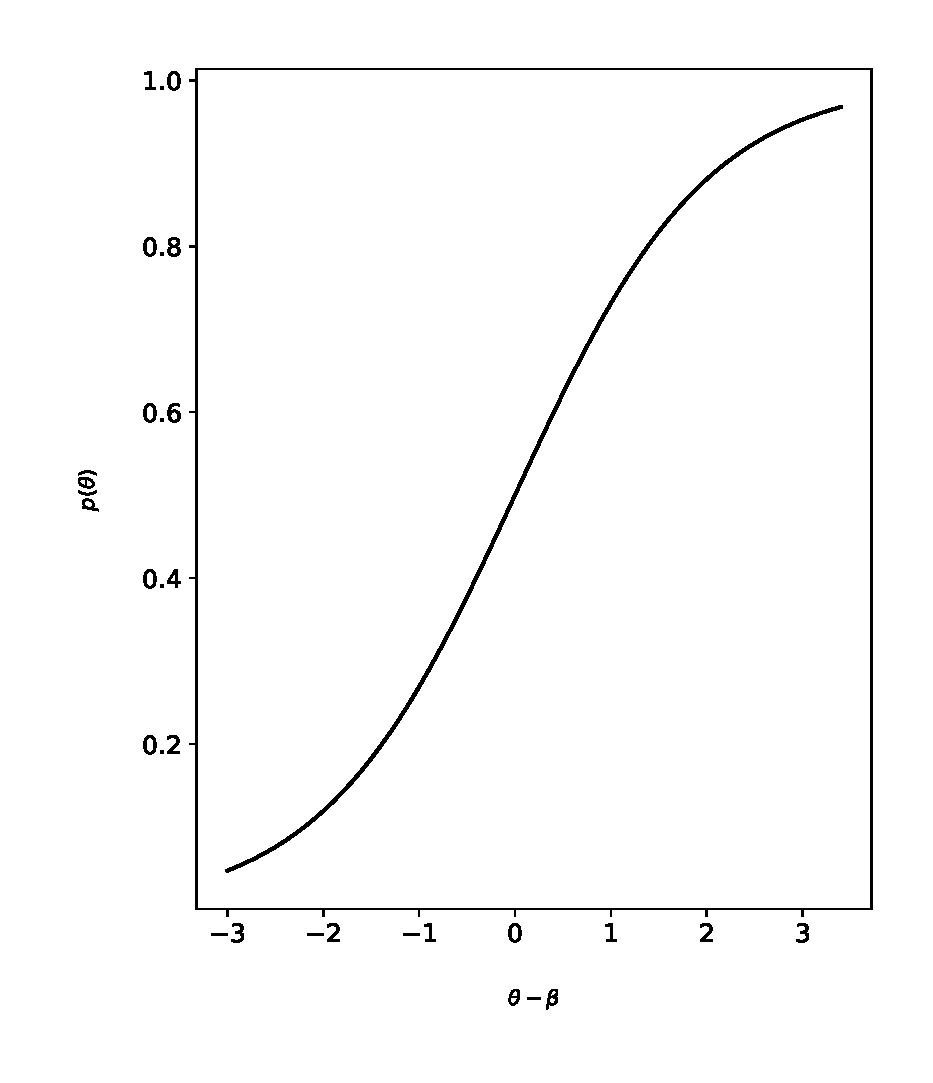
\includegraphics{fig/irt.eps} 
 \caption{A probability curve in Item Response Theory.}
\end{figure}

\begin{figure}[p!]
 \label{fig:mle}
 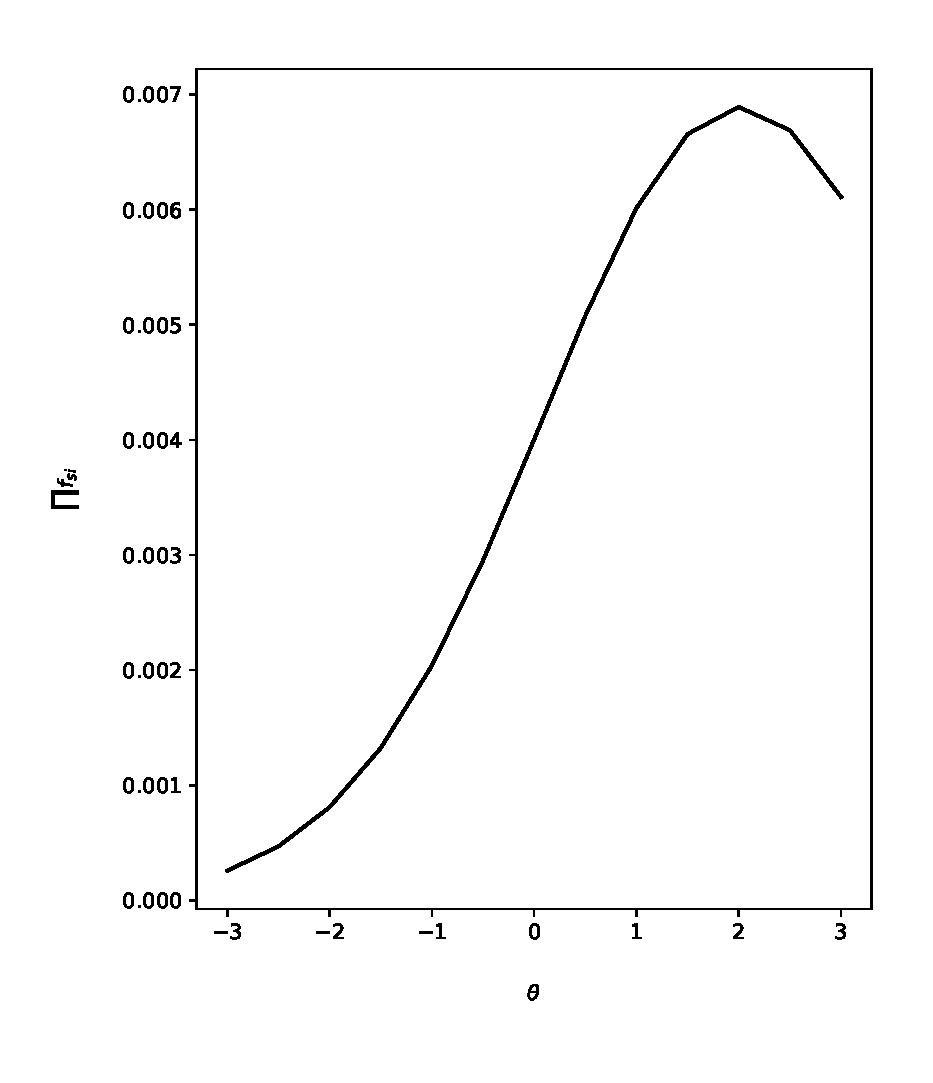
\includegraphics{fig/mle.eps} 
 \caption{A maximum-likelihood estimation for IRT}
\end{figure}

Note that $\alpha_i$, $\beta_i$, and $\gamma_i$ are parameters of the item $i$;
however $\theta_s$ is particular to the student $s$.  

The question difficulty $\beta$ can be estimated by the proportion of students
who pass the question.  The value $\beta$ is analogous to standard deviation in
classical test theory.  If a model of student ability based upon the number of
standard deviations from the mean is desired, and the scores are normally
distributed, then the $\beta$ values can simply be obtained from the
probability density function for a Student's t distribution.

Supposing $\phi$ is the proportion of students who pass the question, $f(v, x)$
is the probability density function for the Student's t-distribution with $v$
degrees of freedom then the relationship between $\phi$ and $\beta$ in such an
assignment would be given by

\begin{equation}
  \phi = \int_{\beta}^{\infty} f(v, x) \ dx
\end{equation}

That is, $\beta$ is the number of standard deviations such that the area from
$\beta$ to $\infty$ under the curve is equal to the proportion of students who
pass the question.  The value can also be obtained from a t-table.

Insofar as the intelligent tutoring system is concerned, the instructor or user
is free to assign $\beta$.  Varying assignments of the $\beta$ scores will
slightly alter the behavior of the system; if a given question is tagged as
easier (that is, assigned a lower $\beta$ value), it will have a greater chance
of appearing earlier in any given student's schedule.

If only $\beta$ is used as a parameter, the resulting model is known as the
1PL or 1 paramter logistic model:

\begin{equations}
 \label{eq:irt}
  p_i(\theta_s) = \frac{1}{1+e^{\theta-\beta_i}}
\end{equations}

\begin{figure}[p!]
 \label{fig:ctt}
 \includegraphics{fig/ctt.eps} 
 \caption{The standard normal curve; the distribution of test scores
  as modeled by Classical Test Theory}
\end{figure}

\begin{figure}[p!]
 \label{fig:pl1}
 \includegraphics{fig/pl1.eps} 
 \caption{The 1PL Item Response Theory model, where $\beta$=1}
\end{figure}


The item discrimination, $\alpha_i$, is defined as the Pearson product-moment
correlation coefficient between the item responses and the composite score on
the test.  Since the item responses are dichotomous, a correlation known as the
point-biserial correlation is computed.  It is defined as:

\begin{equations}
  \alpha_i = \frac{M_1 - M_0}{s_n} \sqrt{\frac{n_0 n_1}{n^2}}
\end{equations}

where $M_1$ is the mean composite score for all correct responses; $M_0$ is the
mean composite score for incorrect responses; $n_0$, $n_1$, and $n$ are number
of incorrect, correct, and total responses, respectively; and the standard
deviation $s_n$ is defined as:

\begin{equations}
  s_n = \sqrt{ \frac{1}{n} \displaystyle\sum_{i=1}^n (X_i - \overline{X})^2} 
\end{equations}

where $X_i$ is the ith response and $\overline{X}$ is the mean of the
responses.  $\alpha$ values have range $[-1, 1]$.  Positive values indicate
that the question is positively discriminating; it is a question which is
useful for gauging the constructs which the composite score seeks to measure.
Students who succeed on a question with a higher $\alpha$ are more likely to
have higher composite scores.  Likewise, negative values indicate that the
question is inversely related to composite score.  Values near zero indicate
that the question is unrelated.

If only $\alpha$ and $\beta$ are used as parameters, the resulting model is
known as the 2PL or 2 paramter logistic model:

\begin{equations}
 \label{eq:irt}
  p_i(\theta_s) = \frac{1}{1+e^{\alpha(\theta-\beta_i)}}
\end{equations}


The probability of guessing is defined as

\begin{equations}
  \gamma_i = \frac{1}{m_i}
\end{equations}

where $m_i$ is the number of options in a multiple choice question.  It is
assumed that each option is equally likely to be chosen if a student with
very low trait ability were to answer the question; that is, there can be
no allowance for logical process-of-elimination tactics.

Addition of the probability of guessing results in the 3PL model, given
in Eq~\ref{eq:irt}.

If the trait ability of the student is known in addition to the item
parameters, then the probability of a correct response can be calculated.
However, it is more often than not the case that the response set of the
student is known, and trait ability is unknown.  In such a case, a variety of
techniques are deployable.

\begin{figure}[p!]
 \label{fig:pl2}
 \includegraphics{fig/pl2.eps} 
 \caption{The 2PL Item Response Theory model, where the item discrimination 
 $\alpha=.5$ and $\beta=0$}
\end{figure}

\begin{figure}[p!]
 \label{fig:pl3}
 \includegraphics{fig/pl3.eps} 
 \caption{The PL3 Item Response Theory model, where $\alpha=1$ and $\beta=0$,
 and probability of guessing $\gamma=.25$}
\end{figure}

Trait ability in IRT can be obtained using a maximum likelihood estimation
(MLE) method, which finds a maximum-likelihood estimate of $\theta$ by testing
a range of $\theta$ values with the IRT formula \cite{baker2004}.  Later it
will be shown how $\theta$ can be estimated.  Another potential technique is
Newton-Raphson, which in most other applications would be the more efficient
and desirable method \cite{baker2004}.  It will later be discussed why the MLE
method is preferred.

%The utility of IRT is that it requires fewer questions to gauge trait ability
%due to its account of other factors ($\alpha, \beta, \gamma$). It is thus
%reputed to be a more mature means of assessment than CTT.

Until now, the fusion of IRT and Bloom's taxonomy has only existed in the
literature as a possibility \cite{sitthisak}.  This work seeks to reconcile
the two by offering a compatible interpretation of Bloom's taxonomy.
%TODO: (SRB) I don't think this is true. See email I sent you on 1/24/2017.

\subsection{Evaluation of Trait Ability}

Consider a set of content items or questions for which the answer is either
incorrect or correct.  This is true in the case of multiple choice questions
(as well as true-false, which is a subset of multiple-choice questions).

Suppose the student has a response set for content items: 

\begin{equations}
  \label{eq:responses}
  X_s = x_{s1}, x_{s2}, \ldots, x_{si}, \ldots x_{sn}
\end{equations}

Here $X_s$ is the response vector of student $s$, and $x_{si}$ is the
correctness of the response to content item $i$ by student $s$; it is zero if
the response is incorrect, or 1 if it is correct.  

These questions may be of various and sundry discriminations, difficulties, and
probabilities of guessing.  The first question may have $\alpha_1=.5$,
$\beta_1=1$, and $\gamma_1=.25$; the second may only differ in its difficulty,
for example $\beta_2=-1$.  However, it shall be assumed that the set of
content items for which the student has provided responses are for the same
concept and the same Bloom taxonomic level.  The reason for this assumption
will become apparent later.

Recall that the probability $p_{si}$ of student $s$ answering the $i^{th}$
question correctly is:

\begin{equations}
  p_{si}(\theta_s) = \gamma_i + \frac{1-\gamma_i}{1+e^{\alpha_i(\theta_s-\beta_i)}}
  \tag{\ref{eq:irt}}
\end{equations}

Since $\theta_s$ is unknown but the response set is known, one method for
determining $\theta_s$ is by guessing a range of possible values.  First, one
can define a function $f_{si}$:

\begin{equations}
f_{si}(\theta_s) =\left\{
         \begin{array}{ll}
               p_{si}(\theta_s) & \mathrm{if}\  x_{si} = 1 \\
               q_{si}(\theta_s) & \mathrm{otherwise}
         \end{array}
       \right.
\end{equations}
% TODO: (SRB) Do you mean p_{si} above when you type p_i?

where 

\begin{equations}
   q_{si}(\theta_s)  = 1 - p_{si}(\theta_s).
\end{equations}

That is, $f_{si}$ assumes the probability $p_{si}$ if answered correctly and
$q_{si}$ if not answered correctly.  Proceeding on the assumption that each of
the observations (that is, responses in the response set) is independent, the
probablity of observing a total response set given a particular $\theta_s$
value is the product of the probabilities $f_{si}$ for all $i$, $1 \leq i \leq
n$, or

\begin{equations}
  \prod_{i=1}^n f_{si}(\theta_s).
\end{equations}

Supposing that there exists some $\theta_s$ which maximizes this product,
the most likely value for the student's true trait ability $\theta_s$ is
defined by:

\begin{equations}
  \theta_s = 
  \underset{\theta}{\textrm{argmax}}
  \Bigg[ 
  \prod_{i=1}^n f_{si}(\theta).
  \Bigg]
\end{equations}


that is, that value of $\theta_s$ which maximizes the product which gives the
probability of all the observations occuring together, given $\theta$.  To
obtain this, products for a range of possible $\theta$ values are calculated.

In the intelligent tutoring system which has been constructed, there are only
thirteen such values, drawing from the +/- system.  The mapping of grades to
trait ability levels is given in Table~\ref{tab:grades}.  This mapping could
also be applied to difficulty levels of questions.  A ``C question'' is one
which students of average trait ability (and perhaps just more than half the
class) may be expected to answer; an ``A+ question'' is a very difficult
question which students of only A+ ability at the time of asking may be
expected to answer; and an ``F question'' is one which may be used to determine
if a student's trait ability is minimally satisfactory.  This mapping lends to
a intuitive understanding of trait ability--as the familiar letter grade.  An
MLE may thereby effectively grade the student.

% TODO: (SRB) Something should be said about the confidence in the trait
% ability assessment given above. In principle, a letter grade could be
% obtained from 2 questions.

To that end, rather than using a fine-grained MLE, it makes practical sense to
calculate products for these thirteen values of $\theta$, since higher
granularity than the +/- system is not useful for final grade assignment, nor
is necessarily more intuitive for the student or instructor.  Restricting the
products calculated to this set of values also makes sense from an efficiency
standpoint.  The total time complexity of the MLE is linear in the size of the
response set, regardless of the number of guesses in $\theta$; while not
asymptotically reduced from using a smaller step size, it is five times faster
than the typical choice of $10^{-1}$, and fifty times faster than the
fine-grained $10^{-2}$.  A graph calculating likelihoods for MLE is depicted in
Figure~\ref{fig:mle}.

% Talk about gradient descent and Newton-Raphson

The total number of MLE estimations for trait ability throughout a course is
equal to the total number of responses for all questions throughout a course,
which can be quite large; it is proportional to the number of students times
the number of items. 


\section{Previous Literature}

\subsection{Works Mentioning Bloom's Taxonomy and Item Response Theory}

There has been one suggestion by Sitthisak et al.  linking Item Response Theory
with Bloom's taxonomy which interprets Bloom levels as difficulty levels.  That
is, the values of $\beta$ from Item Response Theory are mapped directly to
Bloom levels \cite{sitthisak}.  This suggestion exists in the form of a
proposal to implement a computer-aided tester using Item Response Theory.

Another study identifies difficulty by levels of Bloom's taxonomic levels, and
evidently applies Item Response Theory to scoring of the same questions;
however it is unclear how the Bloom levels are mapped ot Item Response Theory
$\beta$ values, or whether or not the mentioned difficulties were hypothesized
or actual difficulties \cite{osborne2013grounded}.  

It is discussed in Sec~\ref{sec:reconciling} why it is desirable for the
current intelligent tutoring system to maintain difficulty and Bloom levels as
separate entities.

Ghulman et al. may be the closest to a full separation of Bloom's taxonomy and
difficulty, as well as establishing the connection between Bloom's taxonomy and
Item Response Theory, as it categorizes questions by Bloom level before
applying a Rasch model to score them \cite{ghulman2009modern}.  The Rasch model
is a model simpler in nature than Item Response Theory which uses one paramter
and is derived from the data set itself.

\subsection{Categories of Systems}

Conole and Warburton have developed a classification system for such
computer-aided testing tools.  Web-based systems \cite{wang2004web} fall under
networked systems, which in turn fall under computer-based assessment
utilities, which in turn falls under computer-assisted assessment
\cite{conole2005review}.  Conole and Warbuton identify that Bloom's taxonomy is
often used as an outcomes-based categorization tool for questions, and that
Classical Test Theory and Item Response Theory are the two main ways in which
computer-aided systems score questions; however these are mentioned in
isolation.

Bejar distinguishes between two types of systems: deficit assessment and error
analysis \cite{bejar1984educational}.  Deficit assessment is concerned with
finding where a student is lacking (such as in trait ability), and error
analysis with what steps in the problem-solving process the student is making
errors in.  This distinction is similar to Anderson's characterization-based
models versus process-based models in intelligent tutoring systems; where
characterization-based models attempt to create a representation of the
student's strengths, process-based models attempt to simulate the student's
problem-solving processes \cite{anderson}.  The current work would fall
squarely within the realm of Bejar's deficit assessment-type system, or
Anderson's characterization-based model.

\subsection{Memory and Forgetting}

Ebbinghaus is credited with having created one of the first mathematical
memories of rememberance and forgetting \cite{ebbinghaus}.  In particular, he
identified that recall drops off exponentially with time.  Empirical studies
since then have supported his original finding.

John Anderson developed a model for process-based learning which could provide
the foundation for an intelligent tutoring system \cite{anderson}.  He called
this Adaptive Control of Thought-Rational (ACT-R).  In ACT-R, there are goals,
akin to problem statements; and rules, or processes used to solve problems; and
finally facts, or knowledge utilized in the course of applying rules.  In this
regard, the structure of an ACT-R model resembles a logic program.  Anderson
also developed a memory model for ACT-R fact and rule recall loosely based on
Ebbinghaus' recall functions, as well as models of re-activation of knowledge
generalized from his own empirial research.  \cite{bacon2003assessing}


\subsection{Executability} 

Finally, some supplementary work on the executability component of the
intelligent tutoring system has been done \cite{castleberry2011}.  One
component of the intelligent tutoring system allows for arbitrary code to
execute before a question or item is displayed to the student.  This feature
was inspired by earlier work on what are known as executable papers.
Executable papers are academic publications residing inside of a virtual (or
other) machine which have editable codes on the front-end and compilers or
interpreters on the backend.  The front-end codes may be edited, then the
paper may be re-compiled so that results from the codes are substituted back
into the paper.  

This idea was originally intended for use with computational science codes, but
was adapted for statistics codes \cite{castleberry2013}.  It has been
integrated into the present work to allow for sophisticated random-number
generation, and for the nature of the questions and items to change in response
to the student or other contextual data.


\subsection{Reconciling Bloom's Taxonomy with Item Response Theory}
\label{sec:reconciling}

A popular interpretation of Bloom's cognitive levels is that they are
difficulty levels, and that these difficulty levels are fixed
\cite{newman1988effect,oliver2004course,lord2007moving,
johnson2006bloom,fuller2007developing}.  Knowledge is easy; synthesis is hard.
We will call this the Bloom-equals-difficulty hypothesis.

A creative interpretation of this hypothesis is that per-student difficulty can
be explained in terms of the demotion of Bloom levels.  The synthesis \emph{and
therefore difficult} questions, once the solution is obtained, are reduced to
knowledge \emph{and therefore easy} questions.  Certainly, this is one possible
scenario.  However, it does not explain a student's ability to answer
altogether distinct synthesis problems; this is to suggest students engage the
cognitive functions of synthesis, presumably as an effect of learning the use
of those functions.  To maintain that Bloom equals difficulty would either
require sustaining the view that students are able to pass the questions
because of a demotion of the cognitive functions required (which poses a rather
cynical view of cognition and of education); or else some notion of trait
ability--in particular one which offsets difficulty, allowing an increase in
the probability of passing the question.

The latter option takes the shape of a primeval form of Item Response Theory,
mapping Bloom levels to $\beta$.  This is highly convenient for the hypothesis
that Bloom equals difficulty, as it becomes agreeable to evaluation with Item
Response Theory.  Nontheless, there are still several issues with the
hypothesis.

Consider first that exposure to knowledge and knowledge questions causes an
increase in $\theta$, provided the student acquires the knowledge.  According
to Bloom's theory, this would increase the probability of answering
comprehension questions correctly.  This agrees with the theory.  However,
according to Item Response Theory, it would also increase the probability of
answering application questions correctly even if no comprehension-level
questions are asked.  In fact, it is theoretically possible to design tests
with sufficient numbers of knowledge questions to place, for any $\beta$,
$\theta-\beta$ much greater than zero--that is for example to say, asking a
sufficient number of knowledge questions should give the reasonable assurance
that application-level ability is high enough not to bother testing it.

As many educators will no doubt agree, this is not the case. Even if a student
scores exceptionally well on knowledge questions, it gives no such assurance
that the student will score similarly on application-level questions.  Even if
knowledge and application scores are found to be correlated, there may be an
additional underlying factor contributing to both scores (such as
intelligence).  The application level is \emph{qualitatively} different; hence
it needs to be tested in spite of the value of $\theta$.

Second, if the hypotheses is strictly true, then there can exist no
counterexample to the claim.  That is to say that there exists no problem on a
lower Bloom level which is more difficult than a problem on a higher Bloom
level.  To take an example, it would be mistaken to call an application problem
easier than any comprehension problem. 

Counterexmaples with intuitive appeal can be constructed.  Take for-loops for
example.  To ask a student to print out the result of a simple loop which
prints numbers 1 to 10 should present an easy enough task.  This is an
application of the many rules of for-loops, but which does not require creative
synthesis or critical thinking on the part of the student (hence it is an
application problem). 

Consider then asking the student to impose a flowchart over the same code,
including the initialization, condition and update statements and the body of
the loop, and to indicate the start and stop of the loop.  Suppose the student
has seen flowcharts over similar loops before.  This is a test of
comprehension--in particular, comprehension of the internal workings (the
control flow) of the loop.    

The application problem above requires only an intuitive comprehension of the
loop: ``\emph{It prints the sequence from 1 up to 10 in steps of 1}'', the
student may realize.  It demands only shallow comprehension and the rule to be
applied is simple.  In the comprehension problem, on the other hand, a higher
degree of precision in comprehension of the loop is demanded to solve the
problem.  The comprehension problem also depends on mastery of the knowledge,
comprehension, and application of flowchart symbols.  Regardless, explaining
the control flow of the loop in full detail is a more difficult undertaking
than simply printing its output. 

Likewise, it is possible to ask the student to synthesize a loop printing the
first ten powers of two, then ask a comparatively difficult analysis question
in the form of an obfuscated loop code.  Impasses in this situation may be
attributed to a lack of knowledge or comprehension of the constructs used in
the presented code.  In the synthesis problem, the student has the advantage of
using known syntax; it is a ``constructed-response'' type of question, rather
than a closed-form question \cite{kuechler2010performance}. 

Third, by Bloom's own admission, it is possible to skip levels for certain
concepts \cite{bloom1956}.  In this case, the ordinality of Bloom levels
breaks down.  A plausible example is given above.  It is possible to teach how
to obtain the numeric sequences printed by for-loops before covering in full
detail the control flow of the loop.  In that particular case, application of
the rule does not depend on comprehension of the code construct.

Alternative interpretations of Bloom levels distinguish between facility or
difficulty and complexity of a problem \cite{hill1981testing,
thompson2008bloom}.  In such interpreations, the cognitive complexity has an
orthogonal relationship to the item difficulty.  The problem with such
interpretations, however, is that they do not readily explain the moderate
correlation that does exist between mean performance and Bloom level
\cite{hill1981testing}.



\pagebreak
\singlespacing
\chapter{Items and Sets}
\doublespacing
\section{Representing Items}

A database was used to represent items, item sets, students, and student
responses.  A full diagrammatic representation of the database is shown in
Figure~\ref{fig:database}.

\begin{sidewaysfigure}[p!]
 \label{fig:database}
 \includegraphics[width=9in]{fig/database.png} 
 \caption{The database layout.}

\end{sidewaysfigure}

The database contains items of the following nature:

\begin{itemize}

  \item \emph{Content}.  These include facts (which may be arranged into
  paragraphs, subsections, and sections), definitions, diagrams, and source
  codes.

  \item \emph{Assessment}.  These include questions, which may be true/false,
  multiple-choice, code writing, code simulation, short answer, and
  freewriting; also Likert scale items.

\end{itemize}

\subsection{Taxonomic Information}

Any output from this database to the student which is intended to solicit input
from the student has the following ordinal dimensions:

\begin{itemize}

  \item \emph{Difficulty}. Following the +/- grading system, difficulties range
  from -3 (very easy) to +3 (very hard), with 0 being medium. As alluded to
  earlier, difficulty determines the probability that a given student in the 
  class will answer the item correctly.

  \item \emph{Bloom level}.  The Bloom levels of cognitive functioning are
  Knowledge, Comprehension, Application, Analysis, Evaluation, and Synthesis.

  \item \emph{Concept}.  Concepts covered in computer science courses; for
  example in a programming course, these may include: Variables, Expressions,
  Control Structures, etc.

\end{itemize}

Any output to the student also has the following categorial dimensions:

\begin{itemize}

  \item \emph{Context}.  A problem may have a domain-specific context, e.g. it
  may be a problem relevant to biology, chemistry, physics, mathematics, etc.

  \item \emph{Type}.  The problem may be true/false, multiple-choice, short
  answer.

\end{itemize}

Each output may also have a dependency list, that is a list of IDs of, or a
rule describing, other output entries which the student should be exposed to
prior to that output.  For this system, Bloom level, subject domain, concept,
and difficulty are dimensions of a test question.  

It is important to note that the dimensions of the data are not necessarily
limited to the above; an exploratory factor analysis (EFA) could be used to
extend the dimensionality of the data semi-automatically.  This functionality
has not been implemented, but there exists a potential for it.


\subsection{Difficulty vs. Bloom Level}

With this, an alternative hypothesis is introduced: the Bloom cognitive
taxonomic level and the difficulty ($\beta$ value) are two separate properties
of items. Rather than being an indicator of difficulty, the Bloom level
indicates a cognitive dependency relationship to items at lower Bloom levels.

This is made clearer by the fact that Bloom levels are hierarchical: knowledge
is required for comprehension, comprehension is required for application, and
so forth.  At any level, there exists the potential to create items of a
range of difficulties. 

However, the application of Bloom's taxonomy to problems is specific to the
concept being analyzed, and moreover specific to the questions being asked.
The application of mathematical expressions (such as being able to evaluate or
reduce expressions) is different from the application of programmatic
expressions (being able to evaluate or reduce such expressions, bearing in mind
the language-specific rules).  The application of mathematical expressions
depends on the comprehension of mathematical expressions, however the
application problems may be easier once the dependencies are satisfied. 

Thus for every concept, and for every Bloom level, a student may possess a
different trait ability ($\theta$ value).  This explains why students would be
able to skip Bloom levels; in particular this would occur if a question of a
higher Bloom level (e.g. Evaluation) did not depend on the Bloom level
immediately preceding it (e.g. Analysis) but rather some lower level (e.g.
Application).  

A series of experiments have been conducted by the author toward the end of
supporting the hypothesis that Bloom levels represent dependency relationships
rather than difficulty levels \cite{castleberry2016}.  These experiments
consisted of demonstrating various ordering effects.  In the experiments,
questions of different Bloom levels (Knowledge through Evaluation) were asked
in forward and reverse order.  It was shown that forward-order schedules
resulted in statistically significantly greater performance than reverse-order
schedules \cite{castleberry2016}.   These experiments are detailed in
Sec~\ref{sec:experiments}.


\pagebreak
\singlespacing
\chapter{Trait Ability}
\doublespacing
\section{Representing Ability}

To form a statistical basis for content scheduling, the measure of trait
ability should be done per-concept and Bloom level.  Therefore if there are $m$
concepts and $n$ levels, there are then $nm$ number of $\theta$ values.  This
shall be called $\Theta$, the trait ability matrix; and $\Theta_s$ will denote
the trait ability matrix of student $s$.  Let $j$ be the index of a Bloom level
and $k$ be the index of a concept, then:

\begin{equation}
\Theta_s =\left[
         \begin{array}{lllll}
              \theta_{s11} & \ldots       & \ldots       & \ldots & \theta_{sn1}  \\
              \vdots       & \ddots       &              &        &               \\
              \vdots       &              & \theta_{sjk} &        &               \\
              \vdots       &              &              & \ddots &               \\
              \theta_{s1m} &              &              &        & \theta_{snm}  \\
         \end{array}
       \right]
\end{equation}

While not strict, there is certainly an ordering about $\Theta$. Lower-level
concepts come before higher-level concepts, and lower Bloom levels come before
higher Bloom levels.  Conceivably a $\Theta$ may look like the following:

\begin{equation}
\Theta_1 =\left[
         \begin{array}{llllll}
             3 & 2.5 & 1   & \y0 & -1     & -2   \\
             2 & 1.5 & \y0 & -.5 & -1.5   & -2.5 \\
             1 &  .5 & \y0 & -1  & -2     & -3   \\
             1 & \y0 & -.5 & -1  & -2.5   & -3   \\
         \end{array}
       \right]
\end{equation}
\vspace{12pt}

Highlighted are areas where $\theta_{sjk} = 0$. These are the areas where the
student has roughly .5 probability of answering a question at difficulty
$\beta=0$ correctly.  Now the question arises: given a rich content item set
with questions in all (Bloom $\times$ concept $\times$ difficulty) categories,
which categories should be selected?  Many factors are taken into account.

\section{Proximal Zone of Development}

Clearly the higher $\theta_{sjk}$ values should be left alone, particularly
those nearing 3, since this demonstrates exceptional mastery of that (Bloom
$\times$ concept) category.  In particular, if $\theta_{sjk} = 3$, there is no
sense in asking at all since trait abilities are capped at 3.  In probabilistic
terms and relative to questions, asking questions for which the estimated
probably is overwhelmingly high, for example $p > .9$, serves no purpose, since
probability estimates of that degree require $\theta-\beta$ significantly
greater than 0.

If $\theta_{sjk} = x$ then it would be ``unfair`` to ask questions in that
category which have $\beta > x$.  According to Equation~\ref{eq:irt}, if $\beta
> x$ and $\theta_s < x$, then $\theta-\beta < 0$ and therefore $p(\theta_s) <
.5$, which means the student has less than .5 probability to answer correctly.
Asking questions for which $p(\theta_s) < .5$ has psychological ramifications,
and potential problems for the updated MLE of $\theta_s$.

It is true that correct answers of more challenging questions raise the ability
returned by a maximum likelihood estimate, however if the probability of
answering them is consistently less than chance and the student responds
accordingly, it is unlikely the estimate will return any $\theta_{sjk} > x$ for
those problems.  Also, given the information $\Theta_s$ about the student, if
it is known that the particular student will more than likely fail a particular
question, it would not make sense to ask it from a psychological standpoint,
provided that the intention of asking is to raise trait ability levels.  If the
student consistently experiences more failures than successes, the student is
more likely to be discouraged by the testing. 
%citation

There is another consideration: the concept tier and Bloom levels.  The course
is a progression of concepts across Bloom levels.  Ideally, the student should
see steady progress in the course.  The set of questions asked at any given
time in a course of study typically range over a subset of concepts.  Testing
for all concepts begins at the Knowledge level; as new concepts are introduced
over time, the tested Bloom level for earlier-introduced concepts rises.  In a
``perfect'' situation, we might observe a trait ability matrix as in
Equation~\ref{eq:perfect}, which shows a clear diagonal reflecting a
progression in both concepts and Bloom levels.  

\begin{equation}
\label{eq:perfect}
\Theta_2 =\left[
         \begin{array}{llllll}
             3   & 3   & 2   &  1 & \y0\\
             3   & 2   & 1   &\y0 & -1 \\
             2   & 1   & \y0 & -1 & -2 \\
             1   & \y0 & -1  & -2 & -3 \\
             \y0 & -1  & -2  & -3 & -3 \\
         \end{array}
       \right]
\end{equation}
\vspace{12pt}

With all this in mind, the most logical subset of (Bloom $\times$ concept)
categories to select questions from are those in the neighborhood of
$\theta_{sjk} = 0$.  One interpretation of this subset is that it is the
student's proximal zone of development.  In the psychology of learning, the
proximal zone of development is the area or areas in which a student can
perform a task with assistance, but could not perform the task without
assistance.  This is consistent with $p \approx .5$.
% citation

However, any question can potentially be asked for any (Bloom $\times$ concept)
category while still placing $p$ at or just slightly above .5 by manipulating
difficulty.  In fact, a matrix of difficulties for desired target questions
could be calculated from the ability matrix:

\begin{equation}
  B_s = \Theta_s - \delta
\end{equation}

where $\delta$ is a sufficiently low value, such as .5.  In the case of
student $s=1$, $B$ would then equal:

\begin{equation}
B_1 =\left[
         \begin{array}{llllll}
             2.5 & 2    & 1   & -.5  & -1.5   & -2.5 \\
             1.5 & 1.5  & -.5 & -1   & -2     & -3   \\
             .5  &  0   & -.5 & -1.5 & -2.5   & -3.5 \\
             .5  & -.5  & -1  & -1.5 & -3     & -3.5 \\
         \end{array}
       \right]
\end{equation}
\vspace{12pt}

Then, it is possible to threshold the matrix so as to eliminate (Bloom $\times$
concept) categories after this stepladder, but include some lag up to and not
including those $\beta_{sjk}$ values for which the student has $\theta_{sjk}$
indicating distinguished mastery:

\begin{equation}
B_1 =\left[
         \begin{array}{llllll}
                 & 2    & 1   & -.5  &        &      \\
             1.5 & 1.5  & -.5 &      &        &      \\
             .5  &  0   & -.5 &      &        &      \\
             .5  & -.5  &     &      &        &      \\
         \end{array}
       \right]
\end{equation}
\vspace{12pt}

From here, the density of questions asked may be in proportion to the distance
from -.5.  Eventually, either the student will reach $\theta_{sjk} = 3$ or else
the tutoring system will run out of questions for that (Bloom $\times$
concept), in which event the trait ability level will stay.

This structure, $\Theta$, therefore shows where to begin asking questions.  It
also helps to define the goal of the intelligent tutoring system: to increase
values in $\Theta$ successively along its diagonal, thereby engineering an
experience similar to course progression.

\section{Updating Ability}

The trait ability matrix must be refreshed (either after a student response,
for a more fine-grained scheduling, or after a total assessment for
course-grained scheduling).  Therefore the student responses must be
auto-graded, and an MLE for each element in $\Theta$ must be performed.

\subsection{Short Answer}

For short answer questions, $\gamma$ is set to 0, since it is assumed that
there are infinitely many possible responses to the short answer question,
unless otherwise indicated in the problem specification. 

Support for auto-grading short answer questions was easily obtained.  Short
answer questions can be graded using the Levenshtein distance, also known as
the edit distance.  Essentially, the Levenshtein distance gives the number of
edits (insertions, substitutions and deletions) required to arrive from the
student input to the solution.  If the Levenshtein distance is below a
threshold, the answer is marked correct; otherwise it is marked incorrect. 


\pagebreak
\singlespacing
\chapter{Item Dependencies}
\doublespacing
\section{Trait Ability Updates}

\subsection{An Assessment Item Autograder}

The autograder for assessment items may be broken into three components, based
on the approaches to autograding: (a) for multiple-choice and true/false, (b)
code writing, (c) short answer and freewriting.  Multiple-choice and true/false
autograding is trivial and will not be discussed. 

\subsubsection{Code Writing Autograder}

Drawing on previous work for a code autograder which uses parsing, the proposed
code writing autograder will consist of a parsing expression grammar (PEG) to
parse keywords and language constructs from source and output files.  The PEG
of choice is Piraha, a simple PEG allowing the creation of easily configurable
plain-text grammar files \cite{brandt2010}.  For the training run, source and output files from
the solutions will be included.  The autograder will use the parse trees to
construct long feature vectors of counts of certain language constructs (e.g. a
count of nested if-statements inside for-loops).  Items will be hand-scored
according to rubrics, where each rubric item corresponds to a portion of the
problem or step in the problem-solving process.  Drawing from previous
work on machine-learning-based autograding, these feature vectors will be
trained on a neural network until a sufficient accuracy on a validation set has
been achieved \cite{shashank2014}. 

\subsubsection{Short Answer Autograder}

The proposed short answer autograder will use a dependency graph alignment
technique \cite{mohler2011} to assign a grade for short answers, but will
investigate alternative scoring methods for computing graph-to-graph alignment,
the potential to score for more than one instructor solution, and the effect of
constraining the allowed length of the response.



\subsection{Updates of Trait Ability from Dependees}
\subsection{Modeling Memory: Updates due to Forgetting}

\section{Dependency Resolution and Item Scheduling}

The general procedure for scheduling content and assessments can be stated as
follows.  In the first iteration, schedule the same content to each student,
then schedule a pre-test. Perform a confirmatory factor analysis on the
pre-test results to ensure that the questions tested the correct concepts;
discard questions whose loadings do not match the concepts the questions were
intended to test.  Measure trait ability $\theta_s$ for each student $s$ for the $B$ Bloom
levels and $C$ concepts tested; then construct a $B \times C$ matrix $\Theta_s$
containing the trait ability estimates for that student.  Then for
$\theta_{s,b,c} < \overline{\Theta}_s$, schedule content of Bloom level $b$ and
concept $c$ from the content pool $X$, to be studied in addition to content
for concepts to be covered.  For the next assessment, randomly sample content
$X_{b,c}$ for each $\theta_{s,b,c} < \overline{\Theta}_s$ in addition to
content covered since the last assessment. If there are no questions remaining
in $X_{b,c}$, let $\theta_{s,b,c}$ stand as the estimate of the student's
trait ability.

\subsection{Finding High-Impact Items}
\subsection{Finding the Next Item: One-At-A-Time Scheduling}
\subsection{Predicting the Final Order: All-At-Once Scheduling}

\pagebreak
\singlespacing
\chapter{Memory}
\doublespacing
\section{Models of Memory}

Ebbinghaus \cite{ebbinghaus} 
\ldots

\begin{equation}
\label{eq:ebbinghaus}
 S(t) = ae^{-bt}
\end{equation}

If $a=1$, this may be interpreted as a probability function:

\begin{equation}
\label{eq:ebbinghaus}
 p(t) = e^{-bt}
\end{equation}

\section{ACT-R}

John Anderson \cite{anderson} 
\ldots

\section{Updates to Memory Model}

\begin{equation}
\label{eq:ebbinghaus}
 p(t) = \frac{1}{1 + e^{m(t-\lambda)}}
\end{equation}

% TODO: memory figure

\section{Re-Activation}

\begin{equation}
\label{eq:ebbinghaus}
 \lambda_n = \rho \lambda_{n-1}
\end{equation}

\subsection{Spacing Effect}

\pagebreak
\singlespacing
\chapter{Scheduling}
\doublespacing
\section{Item Scheduling}

The general procedure for scheduling content and assessments can be stated as
follows.  First, the trait ability matrix for the student is initialized:

\begin{equation}
  \Theta \leftarrow -\infty
\end{equation}

That is, the algorithm initially proceeds on the assumption that it is not
possible for any student to answer any question with probability greater than
zero.  In the first iteration, schedule a preliminary test consisting of a
diagonal block of the trait ability matrix, for example:

\begin{equation}
\Theta_s =\left[
         \begin{array}{llll}
              \y\theta_{s11} & \y\theta_{s21} & \y\theta_{s31} & \ldots \\
              \y\theta_{s12} & \y\theta_{s22} &                 &        \\
              \y\theta_{s13} &                 & \ddots          &        \\
              \vdots          &                 &                 &        \\
         \end{array}
       \right]
\end{equation}

The test should be small enough to be feasible while having enough questions to
support an MLE.  At least two questions are needed per (Bloom $\times$ concept)
for an MLE.  A 3 $\times$ 3 or triangle is sufficient.

Once the data is collected, it is then possible to calculate $\alpha_i$ and
$\beta_i$ for all items. 

With respect to $\alpha_i$, it is desirable to discard any question $i$ for
which $\alpha_i < 0$.  Recall that negative values of $\alpha$ indicate a
negative biserial correlation with the composite score, which means that the
question asked is an indicator of whether or not the student will perform
poorly on the overall measure.  

It $\alpha_i$ is close to -1, then the question may have powerful predictive
power, in which case it should be analyzed for its properties.  It may be
desirable to retain such questions for the purpose of predicting success.
Regardless, if $\alpha_i < 0$, then it along with its subtree should be severed
from the dependency graph, and should only be asked independently as part
of a preliminary testing measure.

With the response set, $\Theta_s$ can be constructed and the proximal zone of
development can be identified, as well as a distribution to select the category
from.  

Once a category is selected, the roots of the assessment tree are traversed
until either a question within the neighborhood of the trait ability is found,
or if no question is found, the traversal ends and another random category is
selected.

\subsection{Finding High-Impact Items}

Once a node on the tree is found, a check is performed to ensure the
dependencies have been asked.  If not, an in-order recursive descent is done on
each dependency, and this procedure is performed on the sub-dependencies.  If
all dependencies have been asked, the probability of the target question is
evaluated.  If the probability is .5, the question is asked. 

If the probability is less than .5, a confirmatory factor analysis is performed
on the dependencies of the node.  At any time, this factor analysis may reveal
a squared loading near zero, which indicates that the dependency relationship
indicated by the graph is not an actual dependency.  In that event, the link
between the target and the ``dependency`` is severed and a confirmatory factor
analysis is re-run on the remaining dependencies.

The most impactful dependency is sought.  This dependency item $i$ is selected
as follows: 

\begin{equation}
  \underset{i}{\mathrm{argmax}} \Bigg[ (1 - p_i) \lambda_i^2 \Bigg]
\end{equation}

The value $\lambda^2$ is the proportion of variance due to that dependency, so
it is preferred to start with higher proportions of variance.  Also $(1-p_i)$
is the room for improvement in the probability of the answering the dependency
correctly.  The intuition is that the more likely it is that the student is
able to answer the dependency correctly, the probability of answering the
target question rises---to the extent of the dependency relationship. 

\subsection{Finding the Next Item}

The maximal value for $(1 - p_i) \lambda_i^2$ may have $p_i < .5$, in which
case the above procedure is recursively applied to the dependencies with
$i$ as the target question.  

Eventually, the algorithm will converge on either a question for which $p_i >
.5$, or it will hit the leaves.  What this means is that there is no question
in the sub-tree for which $p_i$

\subsection{Finding the Whole Schedule}


\pagebreak
\singlespacing
\chapter{Experimental Results}
\doublespacing
\section{Experiments Supporting the Utility of the Taxonomy}
\label{sec:experiments}

\subsection{Experiment 1 Design}. 

Our first experiment tested to see if there is a performance difference between
computer-based assessment and paper-based assessment when questions are ordered
by Bloom level.  Our hypothesis was that students taking the computer-based
assessment would fare better than those taking the paper-based assessment
because of the immediate feedback offered by the computer-based assessment.

We designed a test of 10 questions (2 concepts, each concept having questions
over 5 Bloom levels) to give to students\footnote{All questions may be viewed
at: https://steam.cct.lsu.edu/assessment/}. The questions were of
multiple-choice and short-answer format.  There were two knowledge,
comprehension, application, analysis, and evaluation questions.  No synthesis
questions were asked because of the constrained formats allowed by the
computer-based testing framework.  An interrater reliability of 90\% was
determined by two independent raters (the authors), both computer science
educators, who assessed the Bloom levels of the questions.  After a point of
disagreement about an evaluation-level problem, the test was adjusted to yield
an 100\% interrater reliability.

We designed a test of 10 questions (with 2 concepts, each concept having
questions over 5 Bloom levels) to give to students. The concepts tested were on
recursion and binary trees, and were written to be language-independent.  The
questions were of multiple-choice and short-answer format.  There were two
knowledge, comprehension, application, analysis, and evaluation questions.  No
synthesis questions were asked because of the constrained formats allowed by
the computer-based testing framework.  An interrater reliability of 90\% was
determined by two independent raters, both computer science educators, who
assessed the Bloom levels of the questions.  After a point of disagreement
about an evaluation-level problem, the test was adjusted to yield an 100\%
interrater reliability.

Evaluation-level problems are resistant to multiple-choice and short-answer
formats because of the nature of the category.  Our approach was to use
multiple-choice questions of the ``choose the best answer'' format, in which
there are many proposed uses of a concept or language construct, but one stands
out as the most sensible from the standpoint of experts. 

The test resembled a quiz that might be given in the normal course of teaching
the class. At the end of the quiz, the question ``how satisfied were you with
the (paper/computer)-based medium?'' was asked to gauge satisfaction
differences as well.

For this experiment, volunteers were recruited from a Java programming class
for introductory computer science students.  All students volunteered; candy
was offered as an incentive for all the experiments.  We split the classroom
into two groups, matched based on their current grade in the course.  We gave
the control group the paper quiz, and the experimental group the computer-based
quiz.

An answer was scored as totally correct if it coincided exactly with the
solution, and otherwise scored as incorrect. Correct answers were encoded with
1, incorrect with 0.  A composite score was derived by summing these scores
per-student.

\subsection{Experiment 2 Design}

The second experiment tested the effect of ordering the questions by Bloom
level.  For this experiment we designed another test of 10 questions (2
concepts, each concept having questions over 5 Bloom levels).  This test also
covered recursion and binary trees. In the control condition, questions were
given in forward Bloom-level order.  In the experimental condition, they were
given in reverse order.

For both Experiments 2 and 3, participants were recruited in the same manner;
however for this experiment a C++ class which followed the same conceptual
track was also added to the pool. Matched-pairs were assigned to each group
bsaed on their current grade in each course.  The test was constructed and
interrater reliability gauged in the same manner, and the test was also scored
in the same manner.

\subsection{Experiment 3 Design}. 

The third experiment tested the effect of intervening questions on the
performance of later questions in the assessment.  Our hypothesis was that
overall performance would be improved if incorrect answers triggered the
addition of new {\em intervention} questions from a lower Bloom level.

Experiment 3 participants were recruited from a different class. The test was
this time language-dependent (MATLAB) and tested mastery of control structures,
in particular for-loops.  In the control condition, the control group was given
an assessment of 10 questions, with 2 questions per the first five Bloom
levels. The experimental group was given an adaptive measure.  If at any point
a student answered a question incorrectly, then a question at the next lowest
level was given.  This applied to all levels except knowledge.  So for example
if a student answered an application-level question incorrectly, a
comprehension-level question (related to the application-level question) was
scheduled before another application-level question of the same type.  The
experimental group thus had a a maximum of 4 additional questions asked for a
total possible 14-question test.

\section{Analysis and Results}

\subsection{Experiment 1 Analysis} 

The experimental condition ($N$=27 $M$=6.21) did in fact show a higher mean
score than the control condition ($N$=27 $M$=5.23) in overall performance.
Statistical significance was tested with a one-tailed two-sample matched-pairs
Student's t-test on the composite score. The result indicated a statistically
significant difference ($t$=2.024, $p$=0.048).  The experimental condition
($M$=4.93) showed a higher mean score than the control condition ($M$=4.38) in
satisfaction as well; a similar t-test was done and was marginally
statistically significant ($t$=1.7753, $p$=0.082).  


\subsection{Experiment 2 Analysis} 

The experimental condition ($N$=48, $M$=4.94) showed a higher mean score than
the control condition ($N$=48, $M$=4.31).  Statistical significance was tested
with a one-tailed parametric Student's t-test on the composite score.  The
result indicated a statistically significant difference ($t$=2.13, $p$=0.036).

\subsection{Experiment 3 Analysis}

To tell the immediate effect of the intervention questions, one-tailed
parametric Student's t-test on the composite score of questions starting after
the first intervention question was done. It was hypothesized that the
experimental condition would perform better on the remainder of the test. The
experimental group ($N$=45, $M$=6.98) outperformed the control group ($N$=45,
$M$=6.23).  The result indicated a marginally statistically significant
difference ($t$=1.7082, $p$=0.092).

\subsection{Limitations of These Experiments}

A few validity concerns are to be pointed out. No random order was given in
Experiment 2 because of a lack of available subjects; hence it cannot be
inferred that forward order is no different from random order. The
experimenters (paper authors) designed the tests. The number of items per test
was small to allow for a conservative testing time.  For Experiment 1,
confounding variables (those other than immediate feedback) may have played a
role in test-taking because the test-taking media were different.


\section{Experiments Supporting the Reconciliation of the Taxonomy with IRT}

\subsection{Experiment 1 Design}

In the first experiment, a selection of 16 multiple-choice questions on topics
in operating systems concepts were asked to a sample group of students (N=54)
in an undergraduate-level operating systems class.  Each question had 5 choices
($\gamma$=.2). These questions were tagged with Bloom levels, and interrater
reliability was calculated between two independent raters with experience in
curricular and course design.  Questions were tagged with hypothesized
difficulty levels, which were targeted to be inversely proportional to the
Bloom levels.  Hence the question author intended for the knowledge questions
to be difficult relative to analysis questions, while still maintaining the
appropriate Bloom category.

\subsection{Experiment 2 Design}

To test this modified theory, another experiment was conducted.  The purpose of
this experiment was to explore the relationship among the probability predicted
by unmodified IRT, the probability predicted by modified IRT, and the
correctness of the actual response.  It was hypothesized that modified IRT
should produce a more accurate output than unmodified due to its account of
dependency relationships.

As in the first experiment, a selection of 16 multiple-choice questions on
topics in operating systems concepts were asked to the same sample group of
students (N=54) in the same manner ($\gamma$=.2).  The questions covered 4
concepts, and each concept had 4 questions, each of different Bloom levels
(Knowledge, Comprehension, Application, Analysis), where each question of a
Bloom level higher than Knowledge was dependent on a question of an
immediately-lower Bloom level (e.g. the Application question was dependent on
the Comprehension question of the same concept).  These questions were asked in
forward Bloom order.  The hypothesized difficulties were held equal across
Bloom levels.

\subsection{Experiment 3 Design}

One question remains: can $p_i^{mod}$ be used in some meaningful way?  Suppose
we wish to maximize the probability that a student answers an Analysis question
correctly, and that this Analysis question depends on an Application question.
For that matter, it may depend on more questions, each of which having its own
degree of relatedness to the depender.

We thus posit a more general form of modified IRT which takes into account
multiple dependencies using factor analysis \cite{kim1978}.  From a factor
analysis, it is possible to obtain the proportion of variance explained by each
dependency by squaring the factor loading.  A factor analysis was performed on
the dependent question using dependees as factors to obtain these proportions
of variance explained.

Those proportions of variance could then be used as part of a more generalized
modification to IRT:

\begin{align*}
  p_i(\theta) &=& (1- (\displaystyle\sum_j v_j)) & \Big(\gamma_i + \frac{1-\gamma_i}{1+e^{\alpha_i(\theta-\beta_i)}}\Big) \\
              &+& \displaystyle\sum_j (v_j)   & \Big(\mathbf{sgn}(r)x_{sj}+\frac{1-\mathbf{sgn}(r)}{2}\Big)
\end{align*}

In this generalized formula, $v_j$ refers to the proportion of variance
explained by the dependee $j$ (the squared factor loading for $j$).  Therefore
the sum of these is the total explained variance; one minus the sum is the
total unexplained variance.  Intuitively the probability is proportional to the
amount of variance explained by a dependee.  On the one hand, if one dependee
explains 90\% of the total variance, and the student answers this dependee
correctly, the probability should depend heavily on whether or not the dependee
was correct.  On the other hand, if the total unexplained variance is 1, this
would imply the dependees are not dependees at all.  In this case, the
probability defaults to the item response theory calculation, which uses the
best available information (trait ability and question parameters).

In our experiment to test the utility of this formula, we first required a
small problem set with one depender and multiple dependees.  The experiment
was intended to test whether or not the asking of highly-dependent questions
increased mean scores.

For this we first required proportions of variance between depender and
dependees.  We created 4 questions, where the 4th question had three dependees.
We then asked some of our students (N=22) to answer all of these questions to
obtain proportions of variance, which are listed in Table~\ref{tab:variance}.  

\begin{table}
\begin{center}
\label{tab:variances}
\caption{Proportions of variance due to questions for Experiment 1}
\vspace{12pt}
\begin{tabularx}{\textwidth}{|X|X|X|X|X|}
                                  \hline
      &\y q1 &\y q2 &\y  q3 &\y q4  \\ \hline
\y $v_j$ &  .02 & .23 & .30 &     \\ \hline
\y M    &  .67 & .66 & .43 & .34 \\ \hline
\end{tabularx}
\vspace{24pt}
\end{center}
\end{table}

The others would receive a combination of questions.  Each student was randomly
assigned to one of eight groups.  Four students received each combination of
three questions, such that 4 received the depender outright, 12 received one of
the three dependees (4 each) before the depender, 12 received two of the three
dependees (6 each) prior, and 4 received all three dependees.  The purpose of
this was to test the effect of exposure of each dependee.  Thus each dependee
question appeared in half of the students' assessments.  The total number of
respondents for the depender was 32, and the total number of respondents for
each dependee was 16.  

\section{Analysis and Results}

\subsection{Experiment 1 Analysis}

Interrater reliability on Bloom levels was calculated to be 93\%.  Means for
each Bloom level are reported below.

\begin{table}
\caption{Item means per Bloom category for Experiment 1 ($M_1$) and Experiment 2 ($M_2$)}
\vspace{12pt}
\begin{tabularx}{\textwidth}{|X|X|X|X|X|}
                                                                 \hline
      & \y Knowledge & \y Comprehension & \y Appplication & \y Analysis \\ \hline
\y $M_1$  &  .42 & .53 & .67 & .82  \\ \hline
\y $M_2$  &  .78 & .62 & .48 & .41  \\ \hline
\end{tabularx}
\vspace{24pt}
\end{table}

One-tailed Student t-tests were performed on the three consecutive pairs of
means.  The mean for comprehension was statistically significantly greater than
the mean for knowledge ($t=2.00$), the same held true for application and
comprehension ($t=2.33$), and analysis and application ($t=2.64$).  These
statistics, in conjunction with the interrater reliability for the assignment
of Bloom levels, support the view that Bloom level and difficulty are
distinguishable.

In light of this data, a modification of IRT was sought in order to account for
the dependency relationships that existed among the questions.  Intuitively,
this modification of $p_i$ should possess the properties that: (a) if a
question $x_j$ is unrelated, $p_i$ should be unaffected; and (b) if $x_j$ is
fully related, $p_i$ should be equal to the response value for $x_j$. 

The degree of relationship may be expressed with Pearson's $r$, where
$r_{ij}=0$ indicates no relationship between $x_i$ and $x_j$ and $r=1$
indicates a full positive correlation.  An even more viable metric is the
coefficient of determination $r^2$, which indicates the proportion of variance
in the depender which is attributable to the dependee.  Intuitively, it is this
proportion of the probability which should be associated with the correctness
of $j$.  The remainder may be left to item response theory.  In the event of a
negative correlation, the response should be opposite.


\begin{align*}
  p_i(\theta) &=& (1-r^2) & \Big(\gamma_i + \frac{1-\gamma_i}{1+e^{\alpha_i(\theta-\beta_i)}}\Big) \\
              &+& (r^2)   & \Big(\mathbf{sgn}(r)x_{sj}+\frac{1-\mathbf{sgn}(r)}{2}\Big)
\end{align*}

The above formula satisfies our needs.  The \textbf{sgn} function gives the
sign of $r$.  For $r=1$, $p_i$ defaults to the correctness of the dependee's
answer (0 or 1, depending on whether or not the dependee was answered
correctly);  and for $r=-1$, $p_i$ assumes the flip of the dependee's answer.
For $r=0$, $p_i$ assumes the form of original IRT.  

In the MLE estimation of $\theta$, we would omit question $j$, since it is
included already in the above formula.


\subsection{Experiment 2 Analysis}

Interrater reliability on Bloom levels was once again calculated to be 93\%.
To test the hypothesis that modified IRT leads to an increase in accuracy, a
t-test on the increase in accuracy of probability was conducted at the .05
significance level.

First the probabilities $p_i^{irt}(\theta)$ (for original IRT) and
$p_i^{mod}(\theta)$ (for modified IRT) were calculated.  Note that each of
these formulas require $\theta$. The value for $\theta$ was calculated
per-student using the MLE method on the first data set.  To determine whether
or not $p_i^{mod}(\theta)$ was on the whole more accurate than $p_i^{irt}$, the
result

\[
  \Delta p_{si} = (2x_{si}-1) (p_i^{mod} - p_i^{irt})
\]

was calculated. Here $p_{si}$ represents the probability that student $s$ will
answer item $i$ correctly.  Then $\Delta p_{si}$ represents the increase in
accuracy of the probability; for example, it is positive if $p_i^{mod} >
p_i^{irt}$ and $x_{si} = 1$.

Finally, to test the effectiveness of $p_i^{mod}$, a one-tailed Student's
t-test was calculated on $\Delta p_{si}$ for the dependee questions (N=648).
The test revealed that $\Delta p_{si}$ is statistically significantly greater
than zero ($t=2.05$), implying that $p_i^{mod}$ indeed produces a more accurate
estimate than IRT alone. 

As the data reveals, the proportion of students who passed a question did not
agree with the hypothesized difficulties.  It was suspected that this may be
due to the effect of item dependencies, which the next experiment investigates
in further detail.

\subsection{Experiment 3 Analysis}  

The analysis of this data required examining the relationship between dependent
response and dependee exposure.

Let $E_{sj}$ be 1 if student $s$ was exposed to $j$, 0 otherwise.  Then, our
hypothesis was that exposure of dependee questions should result in an increase
in the probability that the student answers the depender correctly, in
proportion to the amount of variance explained by the dependee.  Below in the
table is the number of times the depender was answered correctly given
exposure to a set of dependees.  Though the data set is small, there does
appear to be a trend in the data.  A clearer trend can be observed by summing
the number of correct responses per exposure to a given question.

\begin{table}[t]
\caption{ The percent of students who answered the depender correctly
given a particular set of questions (left), as well as the percent of students
who answered the depender correctly given exposure to a given question (right).}
\vspace{12pt}
\begin{tabularx}{\textwidth}{|X|X|X|X|X|}
\hline
\y dependees    & \y \#correct &  \y percent & \y \#correct & \y percent \\ \hline
none         &  1  & .25  &1&  .06 \\ \hline
q1           &  1  & .25  &8&  .50 \\ \hline
q2           &  2  & .50  &10& .62 \\ \hline
q3           &  3  & .75  &11& .69 \\ \hline
q1, q2       &  2  & .50  && \\ \hline
q1, q3       &  2  & .50  && \\ \hline
q2, q3       &  3  & .75  && \\ \hline
q1, q2, q3   &  3  & .75  && \\ \hline
\end{tabularx}
\vspace{24pt}
\end{table}

It is interesting to note that to an extent, the proportions of variance
explained by a given question appear to be co-related to the percentage of
students who answered the depender correctly.  However, the numbers are too
small to draw a definitively conclusion.

Due to the low $N$ in Experiment 3, the results do not present
\emph{conclusive} evidence that the intervention of the dependee questions was
responsible.  However, there is enough preliminary evidence to warrant further
investigation.  If there is an effect, it is suspected that exposure to the
dependee problem solution by the ITS plays a larger role than simply the
question itself.



\pagebreak
\singlespacing
%\chapter{Executability and Reporting}
%\doublespacing
%\input{chapter8}
%\pagebreak
%\singlespacing

%To insert additional chapters, copy the previous five lines, using chapterX as the argument of the 
%\input command for Chapter X, where X=6,7,8,...
\addtocontents{toc}{\vspace{12pt}}
\addcontentsline{toc}{chapter}{\hspace{-1.6em} REFERENCES}
%\begin{thebibliography}{999}
%\vspace{0.9em}
%% A review of computer-assisted assessment, 
@article{conole2005review,
  title={A review of computer-assisted assessment},
  author={Conole, Gr{\'a}inne and Warburton, Bill},
  journal={ALT-J},
  volume={13},
  number={1},
  pages={17--31},
  year={2005},
  publisher={Taylor \& Francis}
}

% Concerned with the creation of objective questions at the higher Bloom levels.
% Outlines a method for doing so.  Shows that objective questions at the higher
% levels can be created.
@article{duke2001using,
  title={Using computer-aided assessment to test higher level learning outcomes},
  author={Duke-Williams, Emma and King, Terry},
  year={2001},
  publisher={{\copyright} Loughborough University}
}

% Stresses the need for a competency model, namely one that uses Bloom's taxonomy of
% educational objectives.  Suggests that information in a competency model can be
% used to personalize assessment.
@article{sitthisak2007towards,
  title={Towards a competency model for adaptive assessment to support lifelong learning},
  author={Sitthisak, Onjira and Gilbert, Lester and Davis, Hugh C},
  journal={Service Oriented Approaches and Lifelong Competence Development Infrastructures},
  pages={200},
  year={2007},
  publisher={Citeseer}
}

% In biology, it is agreed that there is a matter of correctness about the answers
% to higher-order questions.
@article{lemons2013questions,
  title={Questions for Assessing Higher-Order Cognitive Skills: It's Not Just Bloom’s},
  author={Lemons, Paula P and Lemons, J Derrick},
  journal={CBE-Life Sciences Education},
  volume={12},
  number={1},
  pages={47--58},
  year={2013},
  publisher={Am Soc Cell Biol}
}

% The CAT prototype introduced here includes a proficiency level estimation
% based on Item Response Theory and a questions’ database. The questions in the
% database are classified according to topic area and difficulty level. The level
% of difficulty estimate comprises expert evaluation based upon Bloom’s taxonomy
% and users’ performance over time.
% Apparently the difficulty is set to the Bloom level. No scheduler.
@article{lilley2005generation,
  title={The generation of automated learner feedback based on individual proficiency levels},
  author={Lilley, Mariana and Barker, Trevor and Britton, Carol},
  journal={Innovations in Applied Artificial Intelligence},
  pages={14--15},
  year={2005},
  publisher={Springer}
}

% Mentioned IRT and bloom, but it is not clear how these are combined or how
% they are scheduled. It seems that the assessments themselves are scheduled. 
% This is a prototype system.
@article{yarandi2011personalised,
  title={Personalised mobile learning system based on item response theory},
  author={Yarandi, Maryam and Jahankhani, Hamid and Dastbaz, Mohammad and Tawil, Abdel-Rahman},
  year={2011}
}

% examines several multiple choice formats 
@article{haladyna1992effectiveness,
  title={The effectiveness of several multiple-choice formats},
  author={Haladyna, Thomas M},
  journal={Applied Measurement in Education},
  volume={5},
  number={1},
  pages={73--88},
  year={1992},
  publisher={Taylor \& Francis}
}

% empirical support for formative assessment, feedback-based learning
@article{lawton2012online,
  title={Online learning based on essential concepts and formative assessment},
  author={Lawton, Daryl and Vye, Nancy and Bransford, John and Sanders, Elizabeth and Richey, Michael and French, David and Stephens, Rick},
  journal={Journal of Engineering Education},
  volume={101},
  number={2},
  pages={244--287},
  year={2012},
  publisher={Wiley Online Library}
}

% ----------------------------------------------------------------------------------

% Duplicate of my research, more importantly suggests outright that Bloom=difficulty
@article{newman1988effect,
  title={Effect of varying item order on multiple-choice test scores: Importance of statistical and cognitive difficulty},
  author={Newman, Dianna L and Kundert, Deborah K and Lane Jr, David S and Bull, Kay Sather},
  journal={Applied Measurement in education},
  volume={1},
  number={1},
  pages={89--97},
  year={1988},
  publisher={Taylor \& Francis}
}

% Very clear support for the thought that Bloom=difficulty, even used for course difficulty rating
@inproceedings{oliver2004course,
  title={This course has a Bloom Rating of 3.9},
  author={Oliver, Dave and Dobele, Tony and Greber, Myles and Roberts, Tim},
  booktitle={Proceedings of the Sixth Australasian Conference on Computing Education-Volume 30},
  pages={227--231},
  year={2004},
  organization={Australian Computer Society, Inc.}
}

% Very clear support for the thought that Bloom=difficulty
@article{lord2007moving,
  title={Moving students from information recitation to information understanding: exploiting Bloom's taxonomy in creating science questions},
  author={Lord, Thomas and Baviskar, Sandhya},
  journal={Journal of College Science Teaching},
  volume={36},
  number={5},
  pages={40},
  year={2007},
  publisher={National Science Teachers Association}
}

% Support for people thinking that Bloom=difficulty
@inproceedings{johnson2006bloom,
  title={Is Bloom's taxonomy appropriate for computer science?},
  author={Johnson, Colin G and Fuller, Ursula},
  booktitle={Proceedings of the 6th Baltic Sea conference on Computing education research: Koli Calling 2006},
  pages={120--123},
  year={2006},
  organization={ACM}
}

% Support for people thinking that Bloom=difficulty
@inproceedings{fuller2007developing,
  title={Developing a computer science-specific learning taxonomy},
  author={Fuller, Ursula and Johnson, Colin G and Ahoniemi, Tuukka and Cukierman, Diana and Hern{\'a}n-Losada, Isidoro and Jackova, Jana and Lahtinen, Essi and Lewis, Tracy L and Thompson, Donna McGee and Riedesel, Charles et al.},
  booktitle={ACM SIGCSE Bulletin},
  volume={39:4},
  pages={152--170},
  year={2007},
  organization={ACM}
}


% Support for Bloom!=difficulty: facility versus complexity
@article{hill1981testing,
  title={Testing the simplex assumption underlying Bloom's Taxonomy},
  author={Hill, PW and McGaw, B},
  journal={American Educational Research Journal},
  volume={18},
  number={1},
  pages={93--101},
  year={1981},
  publisher={Sage Publications}
}

% Support for Bloom!=difficulty
@inproceedings{thompson2008bloom,
  title={Bloom's taxonomy for CS assessment},
  author={Thompson, Errol and Luxton-Reilly, Andrew and Whalley, Jacqueline L and Hu, Minjie and Robbins, Phil},
  booktitle={Proceedings of the tenth conference on Australasian computing education-Volume 78},
  pages={155--161},
  year={2008},
  organization={Australian Computer Society, Inc.}
}


% Cursory
@article{sitthisak,
  title={Cognitive Assessment Applying with Item Response Theory},
  author={Sitthisak, Onjira and Soonklang, Tasanawan and Gilbert, Lester},
  journal={19th Annual International Conference on Computers in Education},
  year={2011}
}

% Bloom original
@book{bloom1956,
  title={Taxonomy of educational objectives},
  author={Bloom, Benjamin Samuel et al.},
  year={1956},
  publisher={David McKay}
}

% Factor analysis
@book{kim1978,
  title={Factor analysis: Statistical methods and practical issues},
  author={Kim, Jae-On and Mueller, Charles W},
  volume={14},
  year={1978},
  publisher={Sage}
}

% Newton Raphson
@book{baker2004,
  title={Item response theory: Parameter estimation techniques},
  author={Baker, Frank B and Kim, Seock-Ho},
  year={2004},
  publisher={CRC Press}
}

% R can be hooked to paper manuscripts to re-generate scientific findings.
@article{ castleberry2011,
          author    = {Dennis Castleberry}
         ,title     = {The Prickly Pear Archive}
         ,journal   = {ICCS}
         ,address   = {Singapore}
         ,publisher = {Elsevier}
         ,year      = {2011}
}

% ...26 studies were deemed as relevant. The main findings from these studies
% are: i) Bloom’s taxonomy has mostly been applied at undergraduate level for
% both design and assessment of software engineering courses; ii) software
% construction is the leading SE subarea in which Bloom’s taxonomy has been
% applied. The results clearly point out the usefulness of Bloom’s taxonomy in
% the SE education context.
@article{ britto2015,
   author = {Ricardo Britto and Muhammad Usman}
  ,title  = {Bloom’s Taxonomy in Software Engineering Education: A Systematic Mapping Study}
  ,journal= {Frontiers in Education Conference}
  ,address= {El Paso, TX}
  ,publisher= {IEEE}
  ,year   = {2015}
}

% Feedback from the students from both first year and second year reflected a
% positive response concerning their perception of the level on which the
% questions were asked. Regarding the first question, 381 students felt that by
% asking questions on higher levels of Bloom’s taxonomy it enriched their
% learning
@article{ bruyn2011
  ,author = {E de Bruyn and E Mostert and A van Schoor}
  ,title  = {Computer-based testing--the ideal tool to assess on the different levels of Bloom’s taxonomy}
  ,journal= {Interactive Collaborative Learning}
  ,address= {Piesany, Slovakia}
  ,publisher= {IEEE}
  ,year   = {2011}
}

% Bloom's taxonomy as applied to program comprehension was successful
@article{ buckley2003
  ,author = {Jim Buckley and Chris Exton}
  ,title  = {Blooms’ Taxonomy: A Framework for Assessing Programmers’ Knowledge of Software Systems}
  ,journal= {International Workshop on Program Comprehension}
  ,address= {}
  ,publisher= {IEEE}
  ,year   = {2003}
}

% Clustering of tasks using EEG is possible
@article{ chatterjee2015,
   author = {Debatri Chatterjee and rajat Das and Anirhudda Sinha and Shreyasi Datta}
  ,title  = {Analyzing Elementary Cognitive Tasks with Bloom's Taxonomy using Low Cost Commercial EEG device} 
  ,journal= {International Conference on Intelligent Sensors, Sensor Networks and Information Processing (ISSNIP)}
  ,address= {}
  ,publisher= {IEEE}
  ,year   = {2015}
}

% Preference for higher-order cognitive activities
@article{ goel2004,
   author = {Sanjay Goel and Nalin Sharda}
  ,title  = {What do engineers want? Examining engineering education through Bloom's taxonomy}
  ,journal= {Australasian Association for Engineering Education}
  ,address= {}
  ,publisher= {}
  ,year   = {2004}
}

% Context-aware vs. lexical schema
% Successful application to system
@article{ kelly2006,
   author = {Tara Kelly and Jim Buckley}
  ,title  = {A Context-Aware Analysis Scheme for Bloom's Taxonomy}
  ,journal= {International Conference on Program Comprehension}
  ,address= {}
  ,publisher= {IEEE}
  ,year   = {2006}
}

% several points aobut requirements
%  formal language
%  typing system
%  Bloom's semantics
@article{ loria-saenz2008,
   author = {Carlos Loria-Saenz}
  ,title  = {On Requirements for Programming Exercises from an e-Learning Perspective}
  ,journal= {}
  ,address= {}
  ,publisher= {}
  ,year   = {2008}
}

% increase in motivation
% comprehension testing fosters code reading
@article{ losada2008
  ,author = {Isidoro Hern\'{a}n-Losada}
  ,title  = {Testing-Based Automatic Grading: A Proposal from Bloom’s Taxonomy}
  ,journal= {International Conference on Advanced Learning Technologies}
  ,address= {}
  ,publisher= {IEEE}
  ,year   = {2008}
}

% speaks well for bloom's taxonomy when manually implemented
@article{ mahmood2014
  ,author = {Mahmood Niazi}
  ,title  = {Teaching global software engineering: experiences and lessons learned}
  ,journal= {IET Software}
  ,address= {}
  ,publisher= {}
  ,year   = {2014}
}

% speaks well for use of Bloom's taxonomy in software inspection
@article{ mcmeekin2009
  ,author = {David McMeekin and Brian von Konsky and Elizabeth Chang and David Cooper}
  ,title  = { }
  ,journal= { Conference on Software Engineering Education and Training }
  ,address= {}
  ,publisher= {IEEE}
  ,year   = {2009}
}

% good for novice programmers to dial it down
@article{ shuhidan2011
  ,author = {Shuhaida Shuhidan and Margaret Hamilton and Daryl D'Souza }
  ,title  = { Understanding Novice Programmer Difficulties via Guided Learning }
  ,journal= {ITiCSE}
  ,address= {Darmstadt, Germany}
  ,publisher= {ACM}
  ,year   = {2011}
}

% My last paper
@inproceedings{castleberry2016effect,
  title={The Effect of Question Ordering Using Bloom's Taxonomy in an e-Learning Environment},
  author={Castleberry, Dennis and Brandt, Steven R},
  booktitle={International Conference on Computer Science Education Innovation \& Technology (CSEIT). Proceedings},
  pages={22},
  year={2016},
  organization={Global Science and Technology Forum}
}


%\end{thebibliography}
\doublespacing
\bibliographystyle{plain}
\bibliography{mainfile}

\pagebreak
\singlespacing
\addtocontents{toc}{\vspace{12pt} \hspace{-1.8em} APPENDIX \vspace{-1em}}
\appendix

\chapter{Appendix A: IRB Documents}
\vspace{0.5em}
\includepdf[pages=-1]{irb/exemption-app-signed.pdf}
\includepdf[pages=-1]{irb/proj-description.pdf}
\includepdf[pages=-1]{irb/consent-form.pdf}
\includepdf[pages=-1]{irb/dc-sd.pdf}
\includepdf[pages=-1]{irb/sb-sd.pdf}
\includepdf[pages=-1]{irb/dc-certificate.pdf}
\includepdf[pages=-1]{irb/sb-certificate.pdf}

\pagebreak

% \includepdf[pages=-]{file.pdf}

%If you need to insert additional appendices, copy the previous four lines, using appendixY as the
%argument of the \input commnd for Appendix Y, for Y=C,D,E,...

%Finally, the vita section is created and included in the Table of Contents.
\chapter*{Vita}
\doublespacing
\setlength{\parindent}{1.75em}
\vspace{0.2em}
\addtocontents{toc}{\vspace{12pt}}
\addcontentsline{toc}{chapter}{\hspace{-1.5em} VITA}

 \includepdf[pages=-]{diss-cv.pdf}

\end{document}


